%!TEX ROOT = thesis.tex
\chapter{ Design and Research Methodology }
\section{Introduction}
In this chapter, the process of designing the proposed ensemble ANNs Model is demonstrated. It is also explained the prototype which can apply using the ensemble ANNs model for forecasting the exchange rates. The parameters  which applied for the neural network is explained further in this chapter. The ways in which this project plans to conduct is also mentioned in this chapter. 

\section{Ensemble ANNs Model Design}
For designing a network, there are five steps suggested by \citeA{lawrence:1993}. They can be summarized as:
\begin{enumerate}
	\item Define the problem. Decide the information to use, and the type of network architecture will be necessary.
	\item Gather the appropriate information.
	\item Define the network architecture. Select network inputs and specifies the outputs.
	\item Train the network.
	\item Test the trained network.
\end{enumerate}

\subsection{ANNs Parameters}
Depending on the type of learning algorithm and neural network applied, there are parameters that must be set,  to control the training process.The following parameters are the ones most commonly applied in different network constructions.
\subsubsection{Learning Rate}
Almost all neural network models have a learning rate parameter associated with them. The learning rate is a factor to scale all corrections while learning and is intended to improve the pace of convergence of the network \cite{lawrence:1993}.
In a typical supervised training , a pattern is presented to the neural network. If it makes an incorrect forecasting, then the difference between the desired output and the actual output is used to adjust the weights. The learning rate parameter controls the magnitude of the changes we make when adjusting the connection weights to move them toward the correct value for the current training pattern and desired output.

A large learning rate produces large changes in weights after each pattern is presented, causing large oscillations in their values. Normally training is started with a large learning parameter, and then as training progress, the learning rate is decreased. The idea is to make large corrections initially, and then fine-tune as training reaches the end.

\subsubsection{Tolerance}
The neural network needs a criterion to compare its output with the actual target. This is specified with the tolerance parameter. Tolerance is the percentage scale of the output. A high value of tolerance will have lower bad facts since the permissible error is more. A higher tolerance results in a more accurate neural network at the cost of higher bad facts. 

\subsubsection{Number of Hidden Layers and Neurons} 
Numerous researchers have proposed the rule of thumb for   selecting  the numbers of nodes which a network should have, and as well as the hidden layer so that it will give the best generalization. One hidden layer is used in all the networks in this project because there  have been shown that  one hidden layer is sufficient to approximate most time-series  forecasting \cite{baestaens:1995, pandya:1995}. Many researchers suggest different ways of selecting the number of neurons or nodes in the hidden layer. \citeA{lawrence:1993} suggested that a method to choose the number of hidden layer. His method can be described as below.

\begin{equation*}
	Number\; of\; hidden\; neurons  = \frac {(Number\; of\; inputs\; +\; Number\; of\; outputs)}{2}
\end{equation*}

Moreover, \citeA{baum:1989} suggested  two methods in their paper to select the number of hidden node or neurons.     
\begin{equation*}
	Number\; of\; hidden\; neurons = MAX(Number \; of \; inputs, Number\; of\; outputs) 
\end{equation*}
\begin{equation*}
	Number\; of\; hidden\; neurons = \frac{(Number\;  of\; inputs\; for\; training \;\ast \;  Error\; tolerance )}{(Number\; of\; inputs\; +\; Number\; of\; outputs)}
\end{equation*}

\subsubsection{Performance Measurements}
There are many methods which measure the accuracy of the neural network by calculating the errors between actual outputs and forecasted outputs by the neural networks. There are many methods to calculate the errors. The most widely used methods are mentioned with their mathematical equation.
\\

\textbf{Root Mean Squared Error (RMSE)}\\
\begin{equation*}
	RMSE= \sqrt{\frac {1}{n}\sum_{i=0}^n(forecasted -  actual )^2} 
\end{equation*}

\textbf{Mean Absolute Error(MAE)}\\
\begin{equation*}
	MAE= \frac {1}{n} \sum_{i=0}^n (forecasted - actual)
\end{equation*}

where  n =  size of the forecasted dataset.

For this project, the ensemble ANNs model consists of three neural networks: NN1, NN2, NN3, and a fusion function. Figure 4.1 explains the model in a graphical manner.

\begin{figure}[hbt!]\centering
	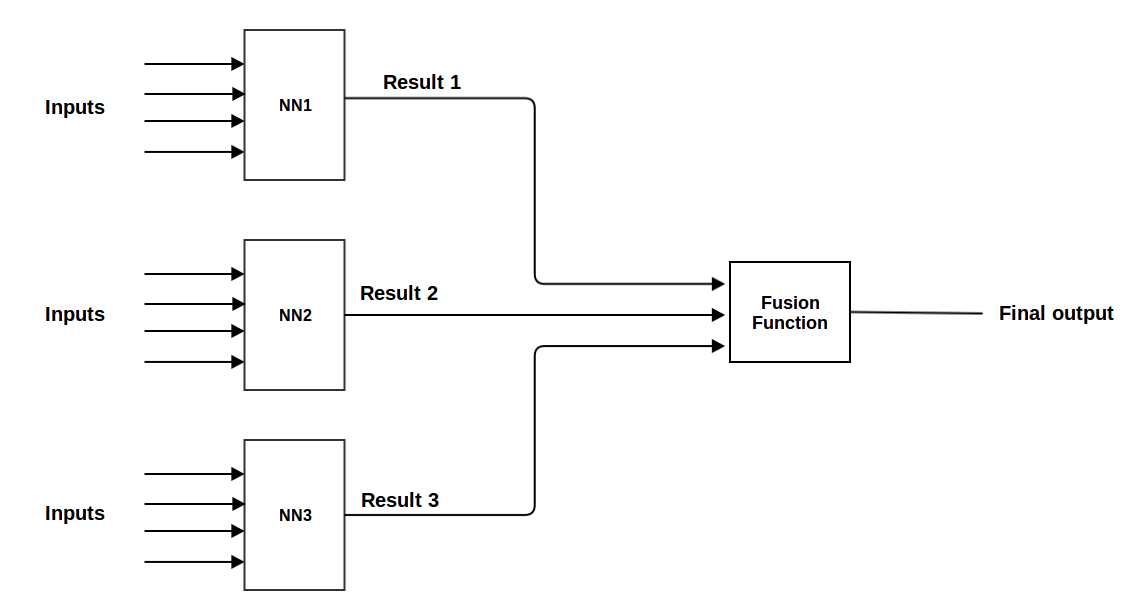
\includegraphics[width=1\textwidth]{ensemblemodel}
	\caption{The proposed ensemble ANNs model}
\end{figure}

Two type of ensemble networks is constructed using this model which are homogeneous ensemble model, and  heterogeneous ensemble model. As for the homogeneous ensemble model, the NN1, NN2, and NN3 is implemented using the same network, MLPs by using different activation functions and learning functions. As for heterogeneous ensemble model, the NN1, NN2, and NN3 is implemented using different ANNs methods such as MLPs, RNN, and RBF neural network. Different type of fusion functions is applied to both model such as average function, minimum function, and maximum function.

The number of inputs is planned to start with prediction order three and increased to ten. The number of hidden layers and hidden nodes is carefully selected  after an extensive review of the previous literature. The outputs from NN1, NN2, and NN3 is used to finalize by using an average function. 

The forecasting is used with  single step prediction with prediction order starting from three which means three days of exchange rates inputs are given to the network to predict the fourth-day exchange rate. In this ensemble, network training starts with a learning rate of 1.0, and as training proceeds, the learning rate is manually reduced to 0.1 and lower. It starts with a tolerance of 0.1 (10\%), and then increase it to between 0.11 (11\%) to 0.14 (14\%) in order to have an acceptable level of bad facts.

\section{Datasets Collection}
Data collection and preparation is the most importance process, and the extensive care is given. The datasets which used to train, validate, and test the ensemble network models are collected from the Bank Negara Malaysia website. The datasets are available from the year 2006 until 2016 in the website. This project utilized the available datasets. Six currencies  such as United State Dollar (USD), British Pound (GBP), Euro (EUR), Swiss Franc (CHF), Australian Dollar (AUD), and Singapore Dollar (SGD) are collected. The data collected are 1 unit of these seven currencies to Malaysian Ringgit.
 
The datasets are processed according to prediction order. For example, if the prediction order is three, then the data set will be processed as three days data as inputs data, the fourth-day data as output data. Table 4.1, 4.2, and 4.3  further showed sample data process for exchange rates from Malaysian Ringgit to other currencies such as USD, EURO, Singapore Dollar (SGD). The Data shown are 1 unit of other currencies to Malaysian Ringgit.

\begin{table}[h!]
	\centering
	\begin{tabular}{|p{2cm}  |p{1.5cm}|p{1.5cm}|p{1.5cm}|p{1.5cm}|}
		\hline
		\multicolumn {5}{|c|}{\textbf{Inputs Data}} \\
		\hline
		\textbf{Day}    & \textbf{Date}  & \textbf{USD} & \textbf{EURO} & \textbf{SGD}\\
		\hline
		\nth{1} Day    & 4/1/2016 & 4.3235  & 4.7003 & 3.0376 \\
		\hline
		\nth{2} Day    & 5/1/2016 & 4.3425  & 4.6986 & 3.0483  \\
		\hline
		\nth{3} Day & 6/1/2016 & 4.3695  & 4.6955  & 3.0527 \\
		\hline
	\end{tabular}
	\begin{tabular}{|p{2cm}  |p{1.5cm}|p{1.5cm}|p{1.5cm}|p{1.5cm}|}
		\hline
		\multicolumn {5}{|c|}{\textbf{Output Data}} \\
		\hline
		\textbf{Day}& \textbf{Date}  & \textbf{USD} & \textbf{EURO} & \textbf{SGD}\\
		\hline
		\nth{4} Day    & 7/1/2016 & 4.4140 & 4.7753 & 3.0754     \\
		\hline
	\end{tabular}
	\caption{Sample Input and Output Data for \nth{4} day }
\end{table}

\begin{table}[h!]
	\centering
	\begin{tabular}{|p{2cm}  |p{1.5cm}|p{1.5cm}|p{1.5cm}|p{1.5cm}|}
		\hline
		\multicolumn {5}{|c|}{\textbf{Inputs Data}} \\
		\hline
		\textbf{Day}    & \textbf{Date}  & \textbf{USD} & \textbf{EURO} & \textbf{SGD}\\
		\hline
		\nth{2} Day    & 5/1/2016 & 4.3425  & 4.6986 & 3.0483  \\
		\hline
		\nth{3} Day    & 6/1/2016 & 4.3695  & 4.6955  & 3.0527 \\
		\hline
		\nth{4} Day    & 7/1/2016 & 4.4140 & 4.7753 & 3.0754     \\
		\hline
	\end{tabular}
	
	\begin{tabular}{|p{2cm}  |p{1.5cm}|p{1.5cm}|p{1.5cm}|p{1.5cm}|}
		\hline
		\multicolumn {5}{|c|}{\textbf{Output Data}} \\
		\hline
		\textbf{Day}& \textbf{Date}  & \textbf{USD} & \textbf{EURO} & \textbf{SGD}\\
		\hline
		\nth{5} Day & 8/1/2016 & 4.3705  & 4.7566  & 3.0472 \\
		\hline
	\end{tabular}
	\caption{Sample Input and Output Data for \nth{5} day }
\end{table}


\begin{table}[h!]
	\centering
	\begin{tabular}{|p{2cm}  |p{1.5cm}|p{1.5cm}|p{1.5cm}|p{1.5cm}|}
		\hline
		\multicolumn {5}{|c|}{\textbf{Inputs Data}} \\
		\hline
		\textbf{Day}    & \textbf{Date}  & \textbf{USD} & \textbf{EURO} & \textbf{SGD}\\
		\hline
		\nth{3} Day    & 6/1/2016 & 4.3695  & 4.6955  & 3.0527 \\
		\hline
		\nth{4} Day    & 7/1/2016 & 4.4140 & 4.7753 & 3.0754     \\
		\hline
		\nth{5} Day & 8/1/2016 & 4.3705  & 4.7566  & 3.0472 \\
		\hline
	\end{tabular}
	
	\begin{tabular}{|p{2cm}  |p{1.5cm}|p{1.5cm}|p{1.5cm}|p{1.5cm}|}
		\hline
		\multicolumn {5}{|c|}{\textbf{Output Data}} \\
		\hline
		\textbf{Day}& \textbf{Date}  & \textbf{USD} & \textbf{EURO} & \textbf{SGD}\\
		\hline
		\nth{6} Day & 11/1/2016 & 4.3985 & 4.8005  & 3.0579      \\
		\hline
	\end{tabular}
	\caption{Sample Input and Output Data for \nth{6} day }
\end{table}
\pagebreak


\section{Research Methodology}

In order to train the network, the historical data sets are required since ANNs models are the class of data-driven approach. Hence, data gathering and data preparation are required. The gathered datasets are also required to separate into three datasets for training, validation, and testing purposes. Figure 4.2 explains the flow of data training, validation, and testing process for the proposed network.
\begin{figure}[hbt!]\centering
	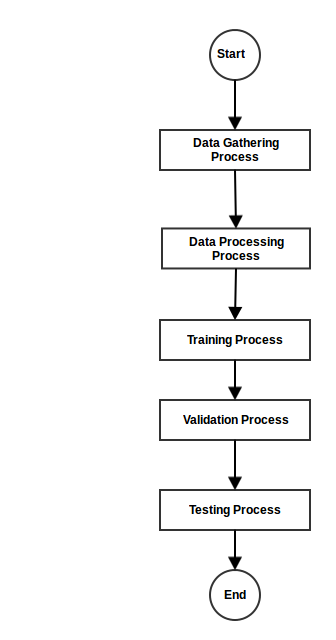
\includegraphics[width=.5\textwidth]{implementation_flow}
	\caption{Implementation Flow}
\end{figure}

Data gathering process is the most important in time series forecasting since it is the class of data-driven approach. Exchange rates between Malaysian Ringgit and other currencies gathered in this process. The historical data sets of exchange rates is collected from Bank Negara Malaysia. The data sets from 2006 until 2016 will be used in this project. 

After data has been collected, it is needed to prepare the data to train the network. The data set are being  divided into training sets, validation set, and testing set.  

The training datasets are being provided to the ensemble network during the training phase. After the network produces the desired model, the ensemble network will be validated using validation datasets. If the ensemble model arrives at the desirable accuracy, then the testing phase will follow using the testing dataset.
\pagebreak

\section{Conclusion}
The process of designing the ensemble ANNs method used different neural networks such as MLPs, RNN, and RBF neural network. Network parameters are chosen carefully based on the suggestions in the literature. Hence, the ensemble methods is constructed and trained for the forecasting the exchange rates.